\section{Ecosistemi Basati su IoTeX}

La blockchain IoTeX supporta una varietà di ecosistemi IoT: shared economy, smart home, veicoli autonomi, supply chain, ecc. Diversi tipi di sviluppatori
sfruttano IoTeX in modi diversi. Gli sviluppatori supportati da IoTeX includono produttori di hardware IoT, sviluppatori di sistemi di controllo dei dispositivi IoT, sviluppatori di app per smart home, produttori di dispositivi per la shared economy, integratori di dati della supply chain, venditori di data crowdsourcing, sviluppatori di automobili a guida autonoma, ecc. Questa sezione descrive alcuni ecosistemi basati su IoTeX.

\subsection{Shared Economy}
Negli ultimi anni, molte aziende si sono concentrate sulla shared economy, dalla condivisione di spostamenti come Uber/Lyft/Didi, la condivisione di alloggi come Airbnb, la condivisione di biciclette come Mobike/ofo, alla condivisione di piccoli oggetti come power bank, ombrelli, ecc... Tutti forniscono
alle persone con una vita migliore, anche se alcuni di loro ricevono un danno dai loro modelli di business. Discutere questi modelli di business riguarda un altro argomento; qui ci concentriamo principalmente sulla loro architettura tecnologica. Tra tutte le economie condivise, la condivisione delle corse in auto è l'unico che non può evitare il lavoro dell'uomo, ovvero il conducente. Non è un'economia basata su IoT. Tuttavia, in futuro, quando la tecnologia delle auto a guida autonoma sarà matura e diffusa, il ride sharing sarà anch'esso basato su IoT.

Tutte le economie condivise basate IoT condividono alcune somiglianze: tutte richiedono una forma di "serratura" che può essere sbloccata da una cauzione, ed un canone di locazione. È assolutamente possibile ed anche efficiente basare l'intero processo di condivisione e restituzione utilizzando un dispositivo IoT. Nel mondo centralizzato, le economie sono basate su un cloud centralizzato. Ci sono vari inconvenienti:

\begin{enumerate}
    \item Un ingente deposito cauzionale è detenuto da una società che potrebbe non essere affidabile. Di recente ci sono stati molti casi in cui l'azienda che gestisce un servizio di bici condivise in Cina non è stata in grado di restituire i depositi ai propri utenti;

    \item Le economie condivise non sono interamente guidate dalla comunità. Molti oggetti condivisi sono di proprietà di un'azienda. Ciò ha causato uno spreco di risorse della società. Prendiam le biciclette condivise come esempio. Quando le aziende di condivisione bici chiudono l'attivita, le bici vengono eliminate.

    \item A causa della natura centralizzata, i dati dell'utente saranno archiviati e controllati da una compagnia. Ci sono rischi che il cloud o il client possano essere violati al fine di ottenere i dati degli utenti.
\end{enumerate}

IoTeX, come infrastruttura, potrebbe essere utilizzato per creare queste applicazioni senza i problemi di cui sopra e rendere le economie condivise decentralizzate e più efficienti. In concreto, un'economia condivisa basata su IoTeX offre i seguenti vantaggi:

\begin{figure}[ht]
    \centering
    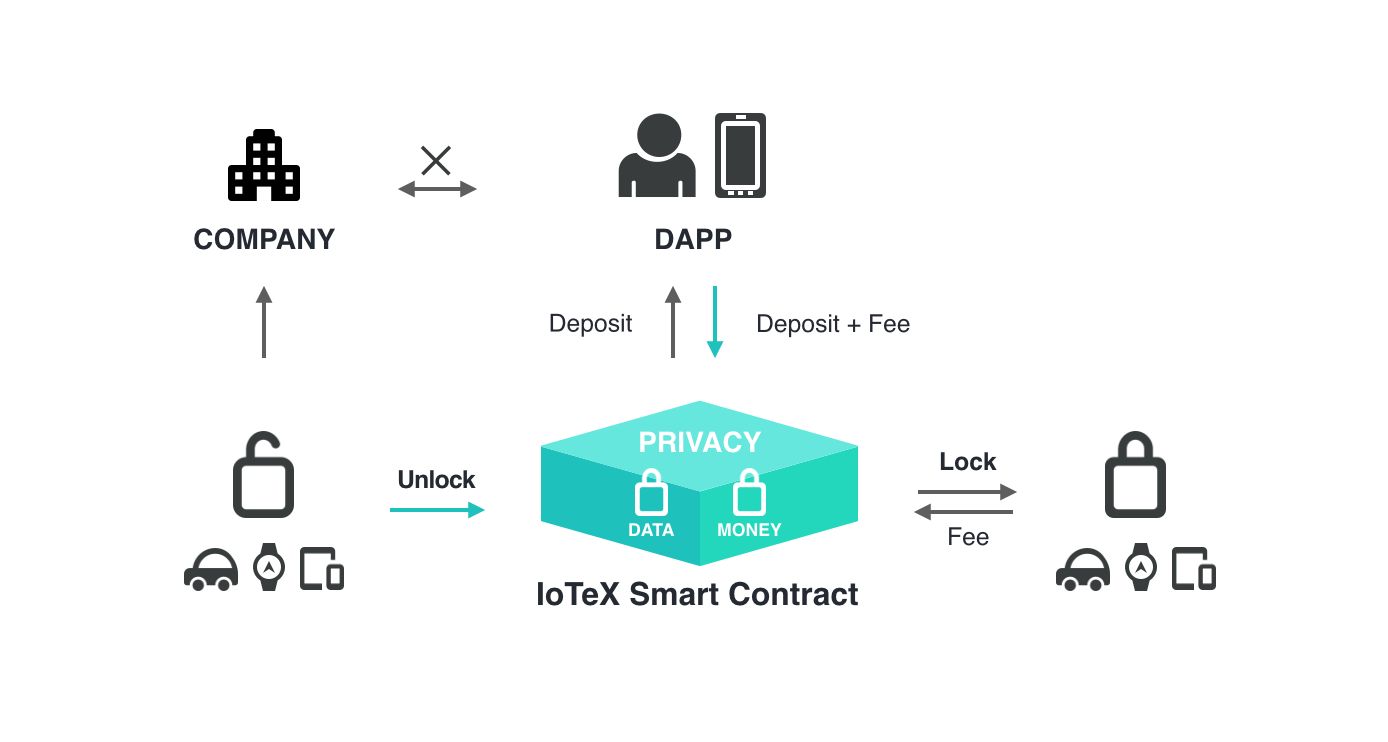
\includegraphics[width=\textwidth]{Figura7}
    \label{fig:Figura7}
    \caption{Shared Economy basata su IoTeX}
\end{figure}

\begin{enumerate}
    \item Il deposito cauzionale è interamente regolato da uno smart contract. Poiché nessuno trattiene i soldi, la restituzione del deposito è sempre garantito. Gli utenti non sono obbligati a fidarsi di una compagnia per utilizzare il servizio.

    \item Ogni oggetto condiviso realizza il suo valore e la sua missione autonomamente. Nell'ecosistema, non importa chi possiede gli oggetti in esso condivisi. Tutti possono possederle e contribuire all'ecosistema. L'economia può essere gestita dalla comunità. Di conseguenza, le aziende possono svolgere il ruolo di manutenere il blocco/serratura IoT e gestire la community. È un modello di business molto più leggero che le aziende possono  espandere velocemente e servire più persone.

    \item Ancora una volta, gli utenti non devono fidarsi dell'azienda per mantenere i propri dati. I dati sono mantenuti nella blockchain con protezione della privacy.
\end{enumerate}

La Figura \ref{fig:Figura7} descrive come funziona la shared Economy basata sulla blockchain IoTeX.

\subsection{Smart Home}

Nel mercato corrente delle smart home, molti produttori di dispositivi IoT continuano a utilizzare tecnologie obsolete per sviluppare i loro prodotti. Hanno bisogno di una grande quantità di lavoro di sviluppo sul loro cloud. Il costo di sviluppo e manutenzione è elevato, e le prestazioni sono basse a causa del viaggio andata/ritorno richiesto verso/dal cloud. Distribuendo i loro prodotti sulla blockchain IoTeX ridurrà in gran parte i costi operativi di ingegnerizzazione e cloud computing e, allo stesso tempo, aumenterà notevolmente le prestazioni dei loro dispositivi. Nel semplice esempio di una lampadina intelligente, con la tecnologia cloud, occorrono due viaggi dal comando dell'utente per cambiare lo stato di una lampadina. I produttori non sono esperti di cloud così spesso il loro servizio non è ottimale. la comunicazione tra andata e ritorno può durare da uno a tre secondi. Ciò li costringe a utilizzare i servizi cloud di grandi aziende IT. Ci sono due aspetti negativi dell'utilizzo di questi servizi cloud:

\begin{enumerate}
    \item I produttori non possono controllare completamente la disponibilità dei servizi cloud.

    \item Hanno bisogno di pagare continuamente per il servizio cloud a fronte di un incasso una tantum per la vendita dei loro dispositivi IoT.

    \item Ci sono rischi di hacking del loro cloud, in caso di hacking lato client o intranet i dati degli utenti verrebbero trafugato oppure si creerebbero problemi di sicurezza domestica.
\end{enumerate}

Al contrario, la blockchain IoTeX gestisce i dispositivi localmente e interagisce con la blockchain pubblica su internet quando necessario. La blockchain pubblica è gestita dalla comunità. Non ci sono costi di manutenzione per i produttori di IoT. La blockchain di IoTeX dispone di protezione della privacy il che può impedire la perdita di dati sensibili o che l'unità di controllo venga hackerata anche se la rete intranet non è sicura.

\begin{figure}
    \centering
    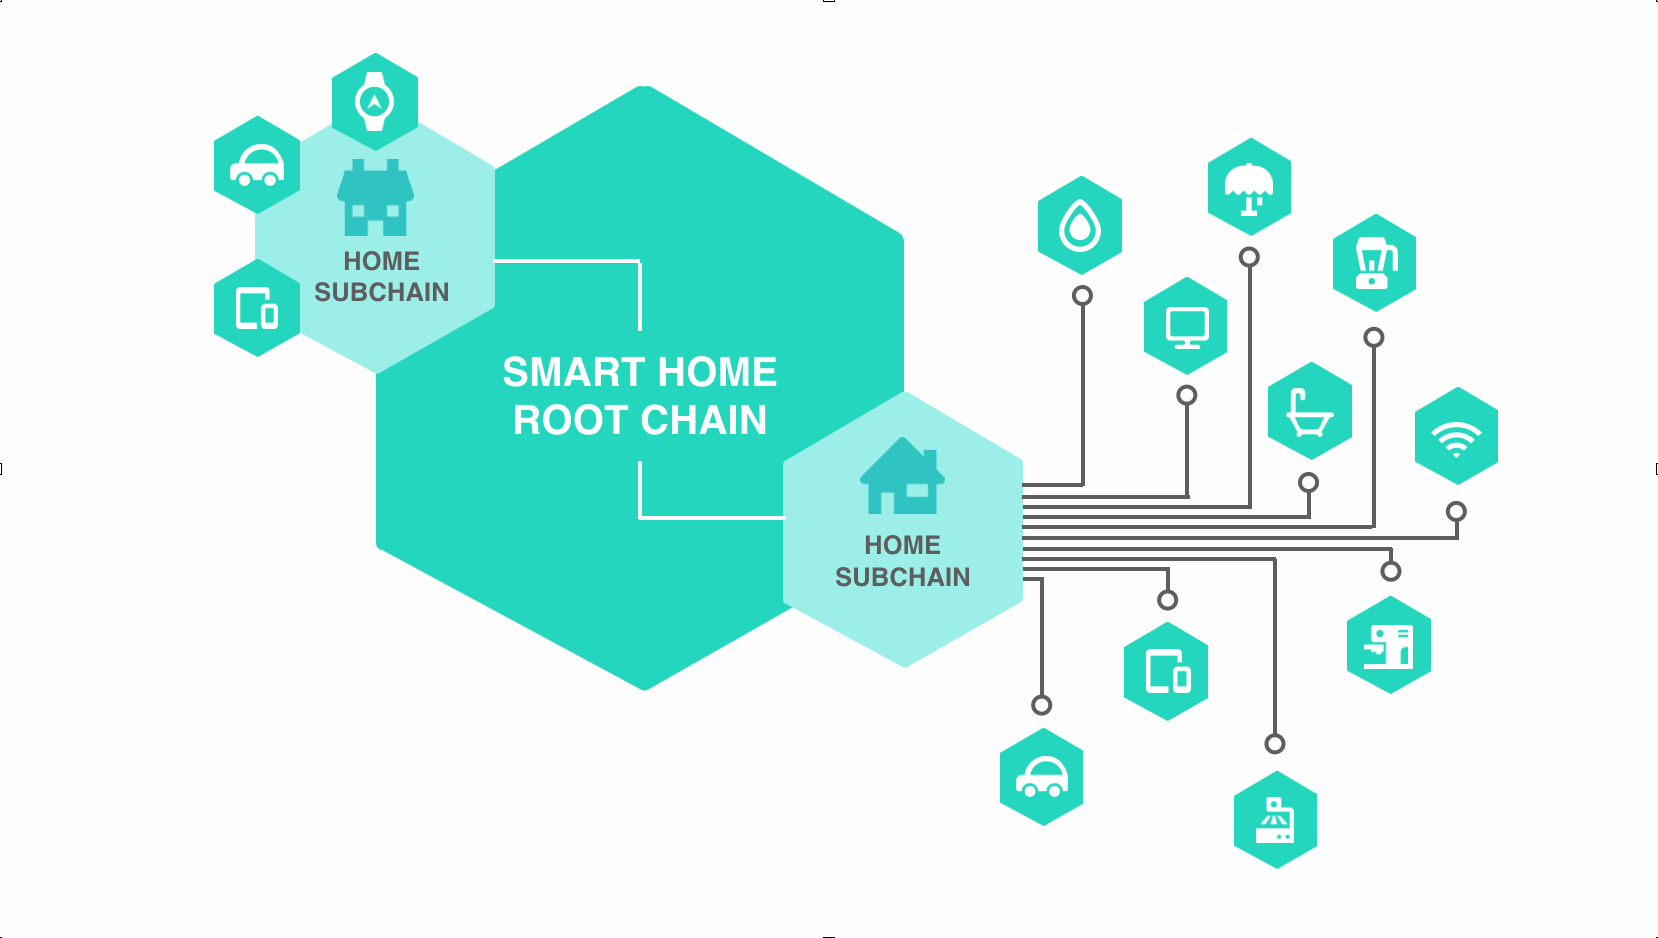
\includegraphics[width=\textwidth]{Figura8}
    \label{fig:Figura8}
    \caption{Smart Home basata su IoTeX}
\end{figure}

Oltre a consentire ai produttori di IoT di implementare i loro dispositivi IoT sulla blockchain IoTeX, IoTeX collaborerà con i produttori di chip IoT per sviluppare chip abilitati all'uso della blockchain IoTeX per accelerare il ciclo di progettazione e produzione di dispositivi IoT. I produttorio di dispositivi IoT semplicemente integreranno il chip per fare in modo che i loro dispositivi siano supportati dlla blockchain IoTeX.


\subsection{Gestione delle identità}
Il mondo in crescita dell'IoT ha avuto un impatto su come la gestione delle identità e degli accessi (\emph{Identity and Access Management} - IAM)
deve funzionare. In termini di identità delle cose, lo IAM deve essere in grado di gestire il sistema utente-dispositivo, dispositivo-dispositivo, e/o dispositivo-servizio. Un modo semplice per la gestione dell'identità è quello di considerare la blockchain IoTeX come un sistema PKI decentralizzato
(grazie alla sua immutabilità) in cui a ciascuna entità viene rilasciata un'identità crittografica sotto forma di certifcato TLS e la chiave privata corrispondente. Questo certificato, che tendenzialmente è di breve durata, viene firmato dal certificato di lunga durata integrato nel dispositivo, e poi pubblicato sulla blockchain IoTeX (rootchain o subchain). I nodi ed altre entità possono accedere e fidarsi del certificato di breve durata ancorato alla
blockchain, e i dispositivi possono quindi autenticarsi quando arrivano online, garantendo sicurezza di comunicazione tra altri dispositivi, servizi e utenti e dimostrare la loro integrità.

Inoltre, è possibile organizzare gerarchicamente i certificati longevi integrati nei dispositivi, come per la PKI convenzionale, in cui i dispositivi genitore possono firmare i certificati dei figli. Grazie alla gerarchia, diventa possibile la revoca e la rotazione dei certificati. Ad esempio, se un dispositivo viene compromesso, il suo dispositivo genitore o anche il dispositivo nonno potrebbero firmare un comando di revoca e inviarlo alla blockchain dove quest'ultimo invalida il certificato del dispositivo.